\section{Introduction}
Nursery inventory from unmanned aerial vehicles (UAVs) is a high-resolution, small-object problem. A single RGB frame may contain many repeated plants, partial crowns, shadows, ground fabric, and row-edge truncation. A detector can localize annotated plants, but converting thousands of local responses into one auditable source-level record still requires decisions about where to inspect, how to reconcile overlapping evidence, and when the available evidence is insufficient. These decisions become more difficult when canopy geometry, plant density, and object scale change across crops.

Compact vision--language models (VLMs) offer a common interface for structured visual questions, but their visual context is poorly matched to 5K aerial frames. Whole-image downsampling can erase small instances; exhaustive tiling repeats overlapping regions and makes VLM cost grow with image size; and syntactically valid outputs can remain visually unsupported. Bounded inference is therefore not merely a deployment convenience: it determines which visual evidence can influence the final decision~\cite{kode2026drone}.

We study the following falsifiable problem. Given a source image and a fixed budget of at most $K$ VLM calls, which regions should be inspected, what source-level inventory record can be supported, and when should the system abstain? OrnaScout separates four responsibilities. A detector supplies inexpensive local evidence over all candidate tiles. A selector allocates the expensive VLM budget. A structured decoder and overlap-aware reducer produce one source record. A validation-fitted gate decides whether that record should be accepted or reviewed. The gate acts after generation and is evaluated as a safety mechanism, not as a source of VLM-call savings.

The agricultural scope is deliberately bounded. The available annotations support plant presence, count-oriented inventory, canopy-density, and annotated-coverage targets. They do not support disease, stress, mortality, quality, or treatment recommendations. The central scientific question is therefore not whether a VLM is an agronomic expert. It is whether structured multimodal evidence provides measurable source-level value beyond detector-only aggregation under a fixed budget and crop shift.

The evaluation uses Magnolia and Azalea as directed visual domains rather than mixing their tiles before splitting. The two crops differ in source-level instance density, normalized object scale, appearance, and spatial organization. All partitions are formed at source-image level before overlapping tiling. The study reports within-crop, cross-crop, and pooled protocols, with uncertainty clustered by source image.

Our contributions are:
\begin{itemize}[leftmargin=*,nosep]
    \item a fixed-budget evidence-allocation formulation that compares detector ranking, true spatial diversity, and controlled exploration at identical VLM cost;
    \item a complete source-level pipeline that contrasts detector-only aggregation with structured compact-VLM inference and overlap-aware reduction; and
    \item a source-disjoint evaluation of directed crop transfer and selective prediction using paired, source-clustered uncertainty and end-to-end efficiency.
\end{itemize}

The contribution is both systems-oriented and empirical: it treats evidence allocation and acceptance as coupled decisions and measures the resulting trade-off among foreground evidence, spatial diversity, negative evidence, accepted risk, review burden, and compute.

\begin{figure*}[t]
    \centering
    \resizebox{\textwidth}{!}{\begin{tikzpicture}[
  font=\sffamily\scriptsize,
  box/.style={draw=black!68, rounded corners=1.2pt, align=center,
    minimum height=9mm, text width=22mm, inner sep=2.5pt},
  compact/.style={box, text width=19mm, minimum height=8mm, inner sep=2pt},
  data/.style={box, fill=blue!5},
  prep/.style={box, fill=cyan!7},
  evidence/.style={box, fill=green!7},
  select/.style={compact, fill=orange!10, draw=orange!72!black},
  vlm/.style={box, fill=violet!7, draw=violet!62!black},
  reliable/.style={box, fill=teal!8, draw=teal!65!black},
  outputbox/.style={compact, fill=gray!6},
  sample/.style={draw=black!70, line width=.45pt, inner sep=0pt, fill=white},
  stage/.style={draw=black!45, dashed, rounded corners=2pt,
    inner xsep=1.4mm, inner ysep=2.5mm},
  flow/.style={-{Latex[length=1.9mm,width=1.35mm]}, line width=.7pt, draw=black!78},
  train/.style={flow,dashed, draw=black!58},
  junction/.style={circle, fill=black!78, inner sep=0pt, minimum size=1.15mm}
]

% Row 1: real cross-crop inputs, source-safe preparation, and local evidence.
\node[sample] (magback) {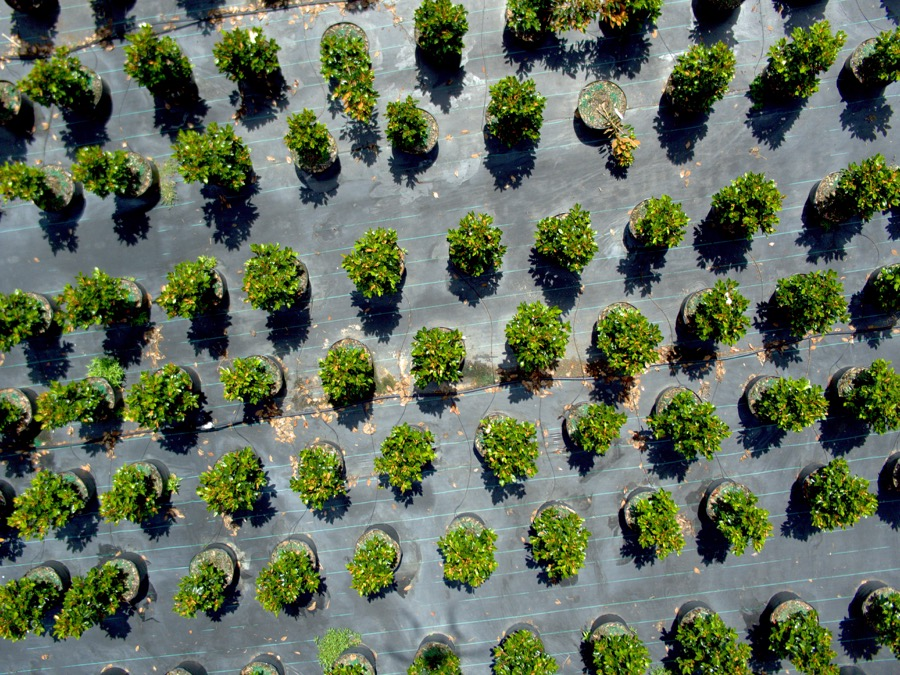
\includegraphics[width=20mm,height=15mm]{figures/input_examples/magnolia_03.jpg}};
\node[sample, xshift=-1.6mm, yshift=1.4mm] at (magback.center) (magmid)
  {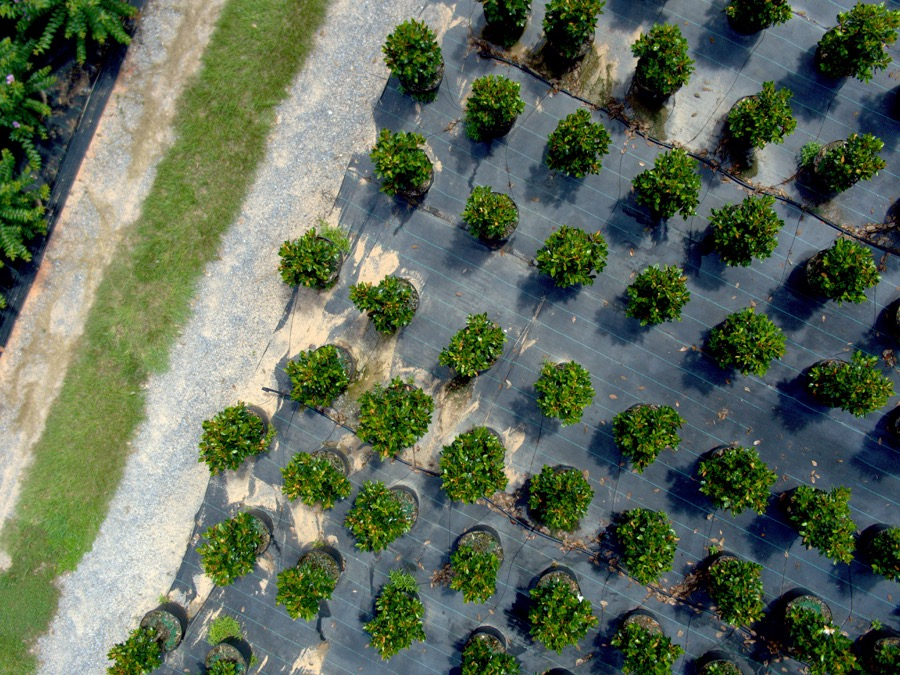
\includegraphics[width=20mm,height=15mm]{figures/input_examples/magnolia_02.jpg}};
\node[sample, xshift=-1.6mm, yshift=1.4mm] at (magmid.center) (mag)
  {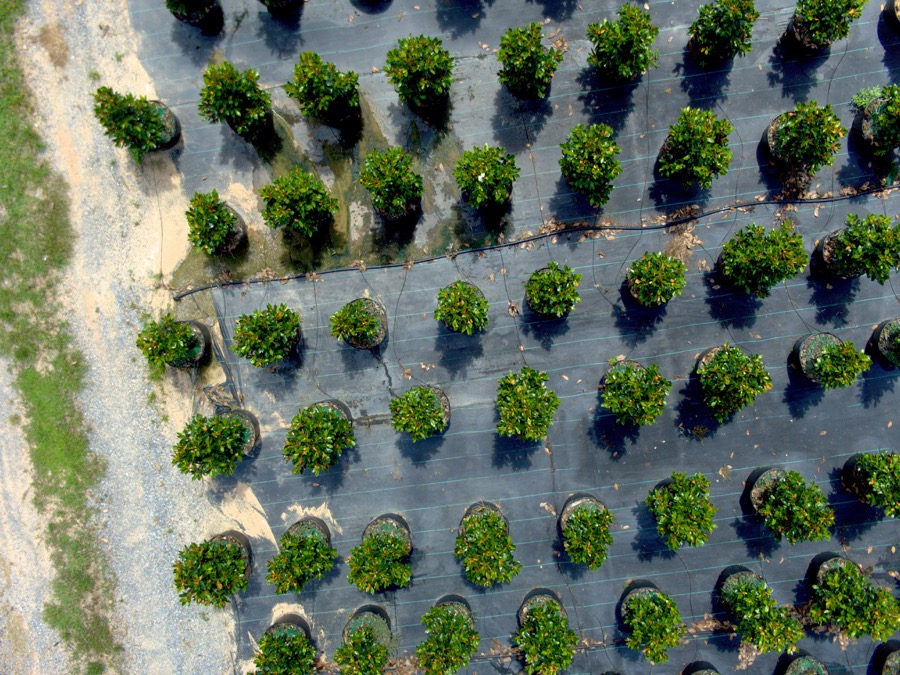
\includegraphics[width=20mm,height=15mm]{figures/input_examples/magnolia_01.jpg}};
\node[fit=(magback)(magmid)(mag), inner sep=.4mm] (magstack) {};
\node[font=\bfseries\scriptsize, above=.7mm of magstack] (maglabel) {Magnolia RGB};

\node[sample, below=8mm of magback] (azaback)
  {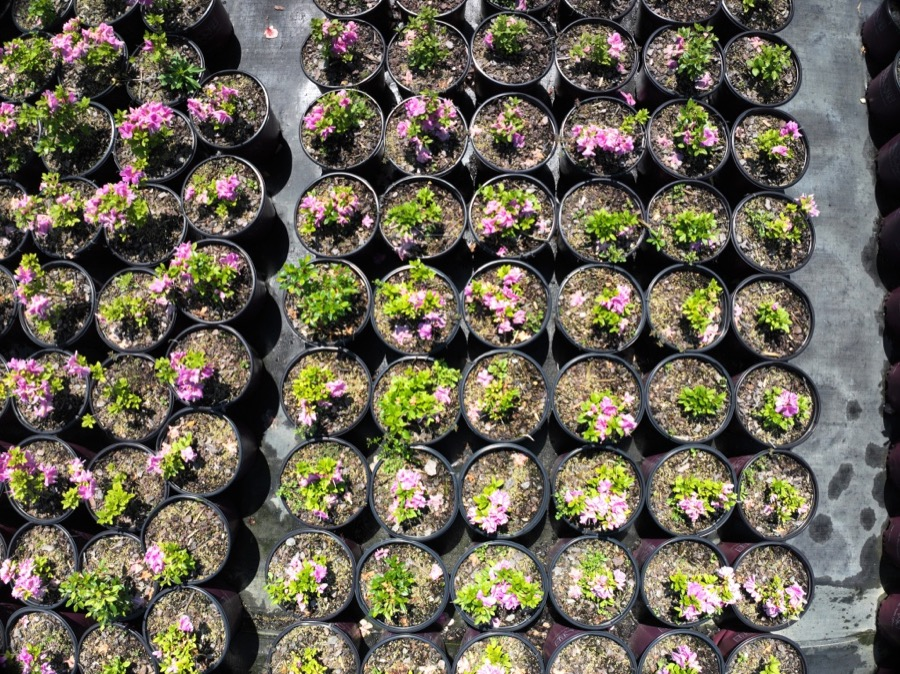
\includegraphics[width=20mm,height=15mm]{figures/input_examples/azalea_03.jpg}};
\node[sample, xshift=-1.6mm, yshift=1.4mm] at (azaback.center) (azamid)
  {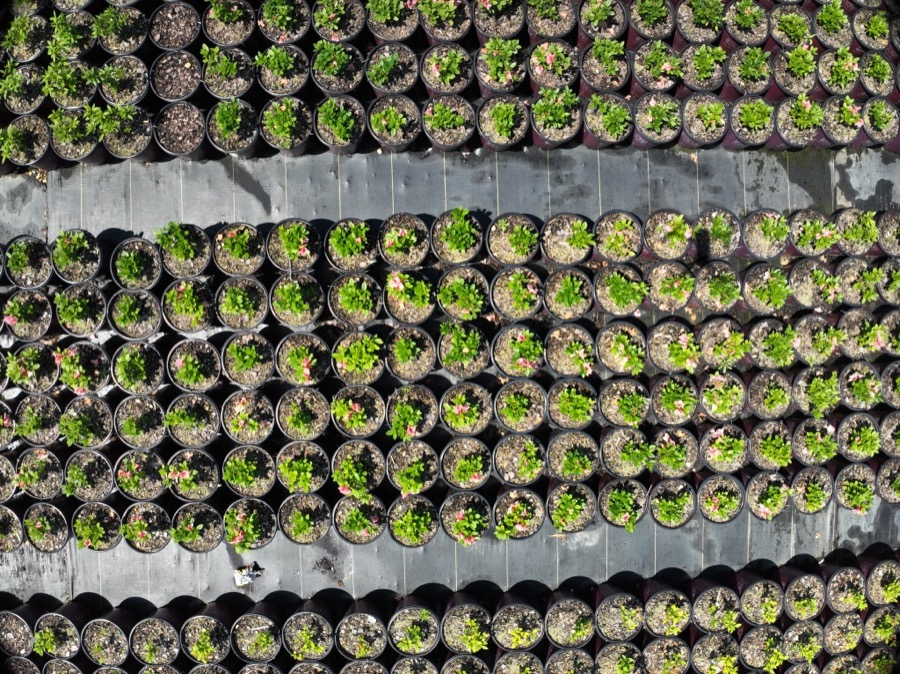
\includegraphics[width=20mm,height=15mm]{figures/input_examples/azalea_02.jpg}};
\node[sample, xshift=-1.6mm, yshift=1.4mm] at (azamid.center) (aza)
  {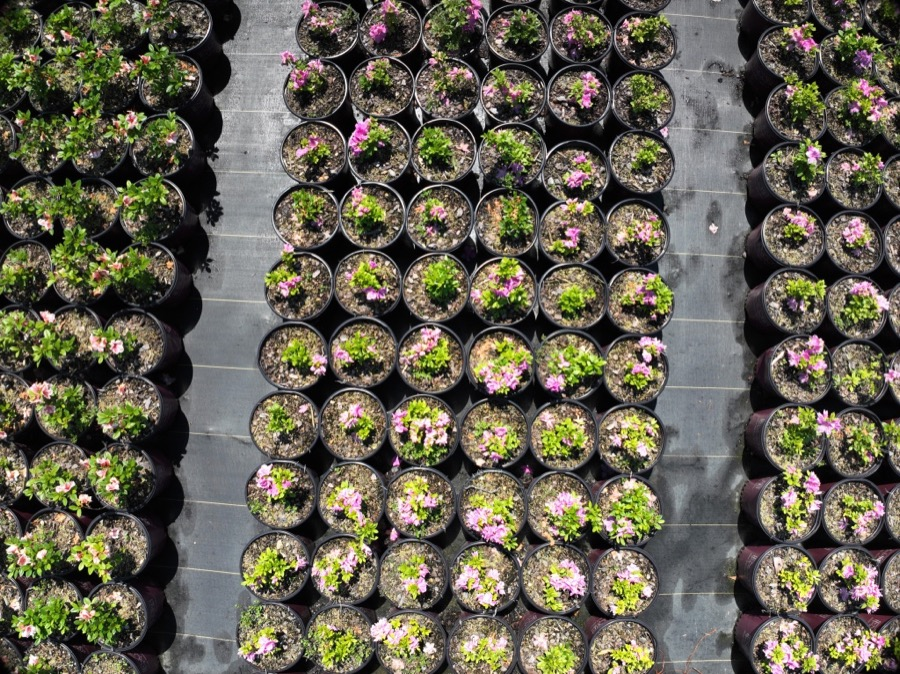
\includegraphics[width=20mm,height=15mm]{figures/input_examples/azalea_01.jpg}};
\node[fit=(azaback)(azamid)(aza), inner sep=.4mm] (azastack) {};
\node[font=\bfseries\scriptsize, above=.7mm of azastack] (azalabel) {Azalea RGB};

\node[prep, right=6mm of $(magstack.east)!0.5!(azastack.east)$] (split)
  {\textbf{Source split}\\train / val / test\\before tiling};
\node[prep, right=5mm of split] (tile)
  {\textbf{Overlapping tiles}\\$s\!\times\!s$, overlap $\alpha$};
\node[evidence, right=5mm of tile] (det)
  {\textbf{Detector evidence}\\confidence $c_t$\\count $n_t$};
\node[outputbox, right=5mm of det, fill=yellow!12, draw=orange!68!black] (labels)
  {\textbf{One-class boxes}\\training / scoring only};

% Row 2: selector, structured inference, and selective output.
\node[select, below=11mm of azastack] (rank)
  {\textbf{Evidence rank}\\$q_t=c_t+\bar n_t$};
\node[select, right=4mm of rank] (allocate)
  {\textbf{Allocate}\\top $K_x$ + explore $K_e$};
\node[select, right=4mm of allocate] (union)
  {\textbf{Budget union}\\$|\mathcal{S}_i|\leq K$};
\node[vlm, right=6mm of union] (adapter)
  {\textbf{VLM adapter}\\SmolVLM2 / Phi\\LLaVA};
\node[vlm, right=4mm of adapter] (schema)
  {\textbf{Schema decoder}\\fixed fields; no\\silent repair};
\node[reliable, right=5mm of schema] (signals)
  {\textbf{Reliability evidence}\\schema, repeats,\\detector agreement};
\node[reliable, right=4mm of signals] (reduce)
  {\textbf{Source reducer}\\overlap-aware\\field fusion};
\node[reliable, right=4mm of reduce] (gate)
  {\textbf{Failure-risk gate}\\validation-fitted\\threshold $\tau^*$};
\node[outputbox, right=4mm of gate, fill=green!8, draw=green!55!black] (accept)
  {\textbf{Accept}\\source record};
\node[outputbox, below=3mm of accept, fill=orange!9, draw=orange!68!black] (review)
  {\textbf{Review}\\abstain / inspect};
\node[outputbox, below=5mm of gate, text width=22mm] (val)
  {\textbf{Validation outcomes}\\observed task failures};

% Boundary-to-boundary paths.
\draw[flow] (magstack.east) -- ++(1.4mm,0) |- ($(split.west)+(0,2mm)$);
\draw[flow] (azastack.east) -- ++(3.0mm,0) |- ($(split.west)+(0,-2mm)$);
\draw[flow] (split.east) -- (tile.west);
\draw[flow] (tile.east) -- (det.west);
\draw[train] (labels.west) -- (det.east);
\coordinate (selectorlane) at ($(rank.north)+(0,2.2mm)$);
\draw[flow] (det.south) |- (selectorlane) -- (rank.north);
\draw[flow] (rank.east) -- (allocate.west);
\draw[flow] (allocate.east) -- (union.west);
\draw[flow] (union.east) -- (adapter.west);
\draw[flow] (adapter.east) -- (schema.west);
\draw[flow] (schema.east) -- (signals.west);
\draw[flow] (signals.east) -- (reduce.west);
\draw[flow] (reduce.east) -- (gate.west);
\node[junction] (gatebranch) at ($(gate.east)+(2mm,0)$) {};
\draw[line width=.7pt, draw=black!78] (gate.east) -- (gatebranch);
\draw[flow] (gatebranch) -- (accept.west);
\draw[flow] (gatebranch) |- (review.west);
\draw[train] (val.north) -- node[right,font=\tiny]{fit on val only} (gate.south);

\begin{scope}[on background layer]
  \node[stage, fit=(maglabel)(magstack)(azalabel)(azastack)(split)(tile)] (stageA) {};
  \node[stage, fit=(det)(labels)] (stageB) {};
  \node[stage, fit=(rank)(allocate)(union), draw=orange!72!black] (stageC) {};
  \node[stage, fit=(adapter)(schema), draw=violet!55!black] (stageD) {};
  \node[stage, fit=(signals)(reduce)(gate)(accept)(review)(val), draw=teal!55!black] (stageE) {};
\end{scope}

% Stage headings are independent of the dashed frames so text never touches a boundary.
\node[font=\bfseries\scriptsize, above=1.1mm of stageA.north]
  {A. Source-safe preparation};
\node[font=\bfseries\scriptsize, above=1.1mm of stageB.north]
  {B. Local evidence};
\node[font=\bfseries\scriptsize, text=orange!55!black, below=1.1mm of stageC.south]
  {C. Budgeted Evidence Selector};
\node[font=\bfseries\scriptsize, text=violet!40!black, below=1.1mm of stageD.south]
  {D. Structured VLM inference};
\node[font=\bfseries\scriptsize, text=teal!38!black, above=1.1mm of stageE.north]
  {E. Selective reliability};
\end{tikzpicture}
}
    \caption{\textbf{OrnaScout overview.} Source images are partitioned before overlapping tiling. A detector evaluates all candidates; equal-budget policies allocate at most $K$ VLM calls. Structured tile records pass through a validation-fitted failure gate and an overlap-aware reducer to form one accepted source record or a review referral. The detector-only path is retained as a controlled baseline. Solid arrows denote deployment computation; dashed arrows denote training or validation-only fitting.}
    \label{fig:architecture}
\end{figure*}
